\documentclass[11pt]{article}
\usepackage[sc]{mathpazo} %Like Palatino with extensive math support
\usepackage{fullpage}
\usepackage[authoryear,sectionbib,sort]{natbib}
\linespread{1.7}
\usepackage[utf8]{inputenc}
\usepackage{lineno}
\usepackage{titlesec}

\usepackage{graphicx,float}
% for setting up equations
\usepackage{amsmath}
\usepackage[usenames,dvipsnames]{xcolor}
\usepackage{gensymb}

\titleformat{\section}[block]{\Large\bfseries\filcenter}{\thesection}{1em}{}
\titleformat{\subsection}[block]{\Large\itshape\filcenter}{\thesubsection}{1em}{}
\titleformat{\subsubsection}[block]{\large\itshape}{\thesubsubsection}{1em}{}
\titleformat{\paragraph}[runin]{\itshape}{\theparagraph}{1em}{}[. ]\renewcommand{\refname}{Literature Cited}

\graphicspath{{/Users/jm200/Library/CloudStorage/Dropbox/Miller Lab/github/ELVI-endophyte-density/Figure/}}
\newcommand{\tom}[2]{{\color{red}{#1}}\footnote{\textit{\color{red}{#2}}}}
\newcommand{\jacob}[2]{{\color{blue}{#1}}\footnote{\textit{\color{blue}{#2}}}}

%%%%%%%%%%%%%%%%%%%%%
% Line numbering
%%%%%%%%%%%%%%%%%%%%%
%
% Please use line numbering with your initial submission and
% subsequent revisions. After acceptance, please turn line numbering
% off by adding percent signs to the lines %\usepackage{lineno} and
% to %\linenumbers{} and %\modulolinenumbers[1] below.
%
% To avoid line numbering being thrown off around math environments,
% the math environments have to be wrapped using
% \begin{linenomath*} and \end{linenomath*}
%
% (Thanks to Vlastimil Krivan for pointing this out to us!)

\title{Variation in the demographic effects of grass-endophyte symbiosis along an aridity gradient }

% This version of the LaTeX template was last updated on
% July 16, 2024.

%%%%%%%%%%%%%%%%%%%%%
% Authorship
%%%%%%%%%%%%%%%%%%%%%
% Please commet out authorship information while your paper is under review. 
% You will need to add this information back in to your final files after
% acceptance.

\author{Jacob K. Moutouama$^{1,\ast}$ \\ 
Julia Martin$^{1}$ \\ 
Ulisses Rizo$^{1}$\\
Malcolm Sherwood$^{1}$\\
Emily Chong$^{1}$\\
Dajanae Pearson$^{1}$\\
Alexandra Jimenez Martín$^{1}$\\
Josh Fowler$^{1}$\\
Ali Campbell$^{1}$\\
Chris Oxley$^{1}$\\
Karl Schrader$^{1}$\\
Tom E.X. Miller$^{1}$\\}

\date{}

\begin{document}

\maketitle

\noindent{} 1. Program in Ecology and Evolutionary Biology, Department of BioSciences, Rice University, Houston, TX USA;

\noindent{} 2. University of Miami, Department of Biology, Miami, Florida;

\noindent{} $\ast$ Corresponding author; e-mail: jmoutouama@gmail.com.

%\noindent{} $\dag$ Deceased.

\bigskip

\textit{Manuscript elements}: Figure~1, figure~2, table~1, appendix~A (for print; including figure~A1, figure~A2, and table~A1), supplemental PDF. Figure~2 is to print in color.

\bigskip

\textit{Keywords}: Examples, model, template, guidelines.

\bigskip

\textit{Manuscript type}: Article. %Or note, natural history miscellany note, comment, reply, invited symposium, featured topic, or historical perspective.

\bigskip

\noindent{\footnotesize Prepared using the suggested \LaTeX{} template for \textit{Am.\ Nat.}}

\linenumbers{}
\modulolinenumbers[1]

\newpage{}

\section*{Abstract}

\newpage{}

\section*{Introduction}

% The journal does not have numbered sections in the main portion of
% articles. Please refrain from using section references (à la
% section~\ref{section:CountingOwlEggs}), and refer to sections by name
% (e.g. section ``Counting Owl Eggs'').

Plant-microbe symbioses are widespread and ecologically important. 
These interactions are famously context-dependent, where the direction and strength of the interaction outcome depends on the environment in which it occurs \citep{fowler2023geographic,hoeksema2015context, bronstein1994conditional}.
Under biotic stress (e.g., herbivory), endophyte symbiosis can benefit host plants by facilitating the production of secondary compounds that deter feeding or cause direct toxicity, thereby reducing insect growth, survival, and oviposition \citep{atala2022fungal,bastias2017epichloe,vega2008insect}.
Similarly under abiotic stress (e.g., drought), symbionts can increase their host tolerance to drought \citep{clay2002evolutionary}.
However, in many plant-microbe interactions, host protection is not guaranteed solely by the presence of a symbionts; rather, the density of the symbiont can determine the effectiveness of this protection \citep{laughton2014combined}. 
Having a greater endophyte density could lead to high resource exploitation by the symbiont, which may be costly (reduction in  growth  or in reproductive) for the host \citep{faeth2009asexual}.
%Thus, plant-microbe  interaction that are beneficial under drought can be parasitic under well-watered conditions \citep{giauque2019endophyte}.
%This cost is often manifested by a reduction in host biomass or reproductive success \citep{faeth2009asexual}, particularly under harsh abiotic conditions \citep{cui2024review}. 
Ultimately, these context-dependent costs and benefits may underlie the observed distribution of host species.

Context-dependence raises the hypothesis that plant-microbe interactions are likely to vary across environmental gradients, from range-core to range-edge, which could have significant consequences for host range expansion.
If the benefits of microbial symbiosis strengthen under environmental stress then symbionts could make range-edge environments more suitable, possibly extending the host’s range limits \citep{allsup2023shifting,rudgers2020climate}.
For instance, fungal endophytes improve the survival of \emph{Bromus laevipes} populations in dry conditions, enhancing their resistance to drought stress at the range edge and thereby extending the species' geographic range \citep{david2019soil,afkhami2014mutualist}.
In contrast, if microbial symbiosis is costly for the host at range edge, then symbionts could limit host range \citep{benning2021microbes,benning2021plant,bennett2022costs}.
%Mutualist limitation reduces population fitness and therefore limits range expansion in \emph{Medicago polymorpha} populations \citep{lopez2021microbial}. 
Although context dependence, along with spatio-temporal variations in abiotic environmental conditions may reduce the effectiveness of the benefits provided by the symbiont to the host species, our understanding of the mechanisms that alter the intensity or likelihood of host-symbiont interactions across host species geographic range is limited.

Ecological studies of plant-microbe symbiosis usually  investigate the interaction from the plant’s perspective and rarely  study how symbiont response to environmental variation might translate to its influence on host demographic performance across host range.
%The presence of symbionts increases host growth and reproduction, outweighing their lower survival rates and resulting in a larger host population size over time.
%Much less is known about how the symbiont respond to environmental variation, and how this might translate to its influence on host demographic performance across host range \citep{garcia2014symbiont}. 
Moreover, studies of plant-microbe symbiosis relied on  methods such as  such as inoculating sterile soil, excluding endophyte fungal hyphae by using fine mesh or rotating cores, and adding fungicide \citep{bennett2022costs}. 
Despite their value, all these approaches are often difficult to implement in field settings or on a large scale.
As a result, the exact mechanisms by which symbionts drive host range limitation and expansion are not well understood, hindering our understanding of the potential cascading effects of symbionts on eco-evolutionary species demography and  range limitation in the context of global change.
%Symbionts are promoting their own selfish fitness by manipulating their hosts' life history traits or resistance to stresses caused by abiotic and biotic variation \citep{kazenel2015mutualistic,giauque2019endophyte,saikkonen1998fungal}. 
%% Plant host–promoted tolerance to these stresses by the fungi may come at a cost.  
%Therefore overlooking the role of symbionts and their potential cascading effects on the eco-evolutionary population dynamics of host species  could lead to inaccurate prediction of host response to current global change. 
% For instance fungal endophyte can reduce plant vital rates (e.g survival) but increase population fitness \citep{rudgers2012there,ahlholm2002vertically}. 

%Understanding how symbiotic interactions are likely to facilitate host persistence in changing environments requires an investigation of the synergistic effects of biotic, abiotic stressors and endophyte presence on individual demographic performance (survival, growth and reproduction) and how that effect can be translated at a population level \citep{bruno2003inclusion,de2006fungal}. 
%One of the best ways to perform that investigation is to use common garden experiments along climatic gradient \citep{schwinning2022common}.
%These common gardens experiments allow the manipulation of variation of biotic and abiotic factors that are likely to change with climate change (eg. temperature, precipitation, endophyte prevalence) and measured species response of such a variation.  

Working across a precipitation gradient in the south-central US, we asked how the demographic effects of endophyte symbiosis varied from core to edge of the host range.
We also asked how does fungal growth affect host demography from range core to range edge. 
To answer, these questions, we studied the symbiotic association between a cool-season grass species (\emph{Elymus virginicus}) and its vertically transmitted fungal symbiont Epichloë elymi. \textcolor{blue}{[Describe ecology and natural history of grass-endophyte interactions]}.
Our experiment was design to test the following hypotheses:
\begin{enumerate}
\item We hypothesized that stress associated with aridity and low precipitation would strengthen the plant-fungal mutualism, such that the fitness benefits of endophyte symbiosis are maximized at the range edge. 
\item We hypothesized that fungal growth in planta varied from range core to range edge. If endophyte growth is limited by host photosynthesis, then environments that are stressful for hosts may correspond to poor endophyte growth. Alternatively, if active regulation by the host is required to keep symbionts “in check”, then environments that are stressful for hosts may correspond to high endophyte growth.
\end{enumerate}

%--------------------------------------------------------------------
\section*{Materials and methods}
\subsection*{Study species}
\emph {Elymus virginicus} (Poaceae) is a cool season perennial grass native to woodland and prairie habitats of eastern North America \citep{shaw2011guide}. 
The westernmost range limits of this species correspond to the longitudinal aridity gradient in the central and southern Great Plains (fig. \ref{fig:site}). 
Throughout its range, the species is  symbiotic with the seed-transmitted fungal endophyte (Epichloë spp.) \citep{rudgers2009benefits}. 
Across natural populations in Texas, endophyte prevalence (fraction of plants that are endophyte-symbiotic) in \emph {Elymus virginicus}  ranged from 10\% to 100\%, with a mean of 53\% \citep{sneck2017variation}. 
Fungal genotyping indicated that the endophytes are capable of synthesizing secondary compounds such as peramine, loline, and ergot alkaloids, which may confer resistance against drought and herbivory \citep{beaudry1951seed}.
In addition, the species is capable of both self-pollination and outcrossing \citep{church1958artificial}. 

\begin{figure}[h!]
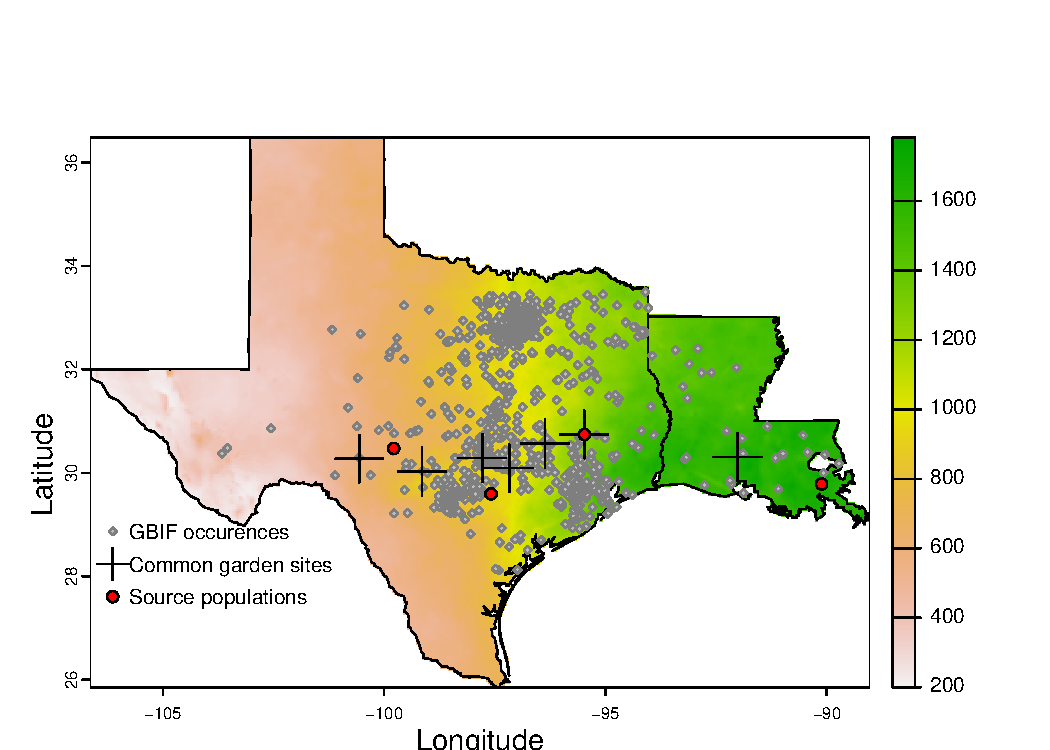
\includegraphics[width=1\textwidth]{clim_map_v1.pdf}
\caption{Distribution of common garden sites across the longitudinal aridity gradient in the central and southern Great Plains. 
Red dots represent the locations of source populations, while grey dots represent the GBIF locations of the species across the study area.}
\label{fig:site}
\end{figure}

\subsection*{Study design}
\paragraph {Experimental Design} 
To understand the demographic effects of endophyte symbiosis from core to edge of the host range, we established  common gardens at 7 sites across the geographic range of \emph {Elymus virginicus} (fig. \ref{fig:site}).
Experimental sites spanned an aridity gradient (temperature gradient).
Common gardens were established in 8 plots per site. 
Plots were 1.5m * 1.5m and the area was tilled of existing vegetation to control for native plant competition.
Plots were also selected in shaded areas under tree canopy or near shrubs to mimic the natural environmental of the species.
In each plot,  we planted 15 individuals  of \emph{E. virginicus} approximately 15 cm deep in an evenly spaced 4*4 grid pattern, with positions randomly assigned. 
For each plot, we randomly assigned a starting endophyte frequency  \jacob{(80\%, 60\%, 40\%, 20\%)}{Do we need a schematic of one replicate
of the experimental design?} and herbivory treatment (herbivores exclusion and herbivores accessibility). 
%Here, the endophyte frequency represents the percentage of  \emph{E. virginicus} individuals that have a symbiont ($E^+$).
We ensured that all plots had comparable quantities of source populations.
After establishing the plots, we watered the plants and recorded initial tiller counts, flowering status and plot position,  endophyte status, source population of each individual plant. 
For herbivory exclusion plots, we enclosed them with 1.2m tall mesh fencing to prevent browsing by vertebrate herbivores and sprayed the plots with insecticide. 
For herbivores accessibility plots (control treatment), we half enclosed the plots with the mesh netting.
We stationed one HOBO MX2307 data logger at each site to collect temperature and volumetric water content in the soil every hour. 

\paragraph {Source populations and Identification of individual endophyte status} 
Plants used  in the common garden experiment were derived from natural populations throughout the native range in the south-central US (fig.\ref{fig:site}, \jacob{Table X}{We need this table  in the Appendix}). 
At each of these natural populations we collected seeds. 
These seeds were planted at Rice University greenhouse.
Seedlings were regularly fertilized every two weeks. 
The seedlings were then vegetatively propagated to produce enough individuals for your experiment (N = 840).
Before planting in the field, we confirmed the endophyte status ($E^+$ or $E^-$) of all  seedlings using either microscopy or an immunoblot assay. 
This was necessary due to the varying success of the heat treatment and differences in the prevalence of endophytes between the natural populations. 
Leaf tissues were stained with aniline blue lactic acid and viewed under a compound microscope at 200x-400x to identify fungal hyphae. 
The immunoblot assay (Phytoscreen field tiller endophyte detection kit, Agrinostics Ltd. Co.) uses monoclonal antibodies that target proteins of Epichloë spp. and chromagen to visually indicate presence or absence. Both methods yield similar detection rates.  


%The vegetatively cloned plants were distributed across all sites intentionally to allow for comparison of endophyte hyphae densities.
\subsection*{Demographic data}
We collected demographic data including survival, growth, and reproduction during June 2023, which coincided with the flowering season of \emph{E. virginicus}. 
On each individual, survival of plants was recorded as a binary (death or alive) and the size of the plant was recorded as the number of living tillers, indicated by the presence of green coloration. 
We recorded the number of inflorescences per plant and the number of spikelets on up to three inflorescences from three reproducing plants.
We limited the spikelets count to three reproducing tillers per plot due to the time consuming nature of this measurement process. 
We used the number of spikelets for these three tillers to estimate the number the average number of spikelets per plants.

%\subsection*{Endophyte density measurements}
%We collected leaf samples from E+ genotypes that were clonally replicated across two or more sites to quantify endophyte hyphal density and test its associations with host genotype and environmental factors. 
%Relying on clonally replicated genotypes for this analysis allowed us to observe the same genetic individuals in different environments, and partition variation in symbiont density between genetic and environmental sources. 
%
%There were seven unique genotypes of E+ hosts (three PALM, three JLP, one SHS) that were clonally replicated across two or more experimental sites. 
%We collected leaf samples from clonal replicates of these genotypes at up to five sites (excluding COL and SON, where no samples were taken) at the time of the demographic census.
%Samples were taken opportunistically based on survival status and size (we avoided leaf collection from small individuals with few leaves that were vulnerable to mortality).
%We collected 20 leaf samples in total, consisting of one genotype replicated at five sites, three genotypes replicated at three sites, and three genotypes replicated at two sites. 
%
%Samples were placed in a cold cooler in the field and then stored in a -20 freezer until processing.
%In the lab, we examined sections of inner leaf sheath for hyphal density. 
%For each sample, four “peels” of the leaf sheath were placed on a single gridded glass slide (including xmm cells), stained with an aniline blue-lactic acid solution, and viewed under a light microscope at X magnification, following methods in \textcolor{violet}{Sneck et al. 2019}. 
%We randomly sub-sampled cells on the gridded slide, skipping those with less than 25\% leaf peel coverage, until we reached 10 cells for each sample, which amounted to a subsample totaling up to 12mm² per leaf.
%We took digital images of each grid cell. 
%Using ImageJ, we set the scale using the microscope reticle to measure the visible area of the leaf peel within the cell and the total length of the hyphae fragments within the leaf peel.
%This yielded an estimate of endophyte density in the units of length (mm) per area (mm2). 

\subsection*{Candidate Models}
To assess how stress associated with aridity and low precipitation affect plant-fungal mutualism, we developed five mixed-effects models for each vital rate. 
Each vital rate was modeled with 10 candidates models. 
These included XXX

In each of the mixed-effects models, we specified two random effects to account for heterogeneity among plot within site and heterogeneity among host source populations. The first random effect was a nested random effect (plot within site) and the second one was a random intercept effect (population). We modeled growth with a Gaussian distribution using the package lmertest  \textcolor{blue}{(Source)}. We modeled fertility (number of spikelet) with a zero-inflated negative binomial distribution using the package glmmTMB  \textcolor{blue}{(Source)}. We preferred the negative binomial in which the variance was modeled as a non-linear function of the mean (variance = m (1 + m/k)). For each vital rate, the first model was the intercept only model which is the null model. The second and the third models regressed vital rate against the additive effect of endophyte status and mean of soil moisture or coefficient of variation of soil moisture. The fourth and fifth models regressed vital rates against the interaction effect of endophyte status and mean of soil moisture or coefficient of variation of soil moisture (Appendix S1). We compared the five models using the Akaike Information Criterion (AIC) to select the best model \textcolor{blue}{(Source)}. 

\subsection*{Model Fitting, Model Selection, and Parameter Estimation}

%%%%%%%%%%%%%%%%%%%%%
% Acknowledgments
%%%%%%%%%%%%%%%%%%%%%
% You may wish to remove the Acknowledgments section while your paper 
% is under review as the Acknowledgments may reveal your identity.
% If you remove this section, you will need to add it back in to your
% final files after acceptance.

\section*{Acknowledgments}

OEC would like to thank Madlen Wilmes, Gyuri Barab\'{a}s, Flo D\'{e}barre, Vlastimil K\v{r}ivan, and Greg Dwyer for their comments and suggestions on this template.

%%%%%%%%%%%%%%%%%%%%%
% Statement of Authorship
%%%%%%%%%%%%%%%%%%%%%
% This section should also be commented out while your MS is undergoing
% double-blind review. The specifics should of course be adapted to
% your paper, but the paragraph below gives some hints of possible
% contributions.

\section*{Statement of Authorship}

OEC conceived the experiments, collected the data, and wrote the original draft.
GHC provided specimens and analyzed the model.
AQE oversaw data analysis and developed the code. 
All authors reviewed and edited the writing at all stages of revision.

\section*{Data and Code Availability}

On initial submission, you may use this section to provide a URL for editors and reviewers that is `private for peer review'. After acceptance, this section must be updated with correct, working DOIs for data and code deposits (such as in Zenodo, Dryad, or DataVerse). An example statement could resemble the following: All data and code for this work are available from the Dryad Digital Repository, \citealt{CookEtAl2015}). 

\section*{Appendix A: Additional Methods and Parameters}

% In most cases, authors should typeset supplementary material in a separate,
% author-supplied PDF. For author-supplied PDFs, please consult the
% AmNat_supp_template.tex document, available from
% https://www.journals.uchicago.edu/journals/an/instruct 
%
% If you want to use cross-references within the supplemental TeX file,
% it may be helpful to \usepackage{xr} and include the command 
% \externaldocument{name-of-supplemental-tex-file}
%
% The Appendix instructions below apply to cases in which
% a brief appendix is to appear in print after the main body of the article.
% That notably includes descriptions of methods, tables defining parameters,
% and other material necessary for reproducing the MS's results.
%
% Please reset counters for the appendix (thus normally figure A1, 
% figure A2, table A1, etc.).
%
% Most AmNat articles have no more than one print appendix. If your article
% has more than one, counters for each appendix should match the letter of
% that appendix. For example, tables in Appendix B should be numbered table B1, % table C2, etc. This applies to tables, equations, and figures.
%
% It's better not to use the \appendix command, because we have some
% formatting peculiarities that \appendix conflicts with.

\renewcommand{\theequation}{A\arabic{equation}}
% redefine the command that creates the equation number.
\renewcommand{\thetable}{A\arabic{table}}
\setcounter{equation}{0}  % reset counter 
\setcounter{figure}{0}
\setcounter{table}{0}

\subsection*{Fox--dog encounters through the ages}

The quick red fox jumps over the lazy brown dog. The quick red fox has always jumped over the lazy brown dog. The quick red fox began jumping over the lazy brown dog in the 19th century and has never ceased from so jumping, as we shall see in figure~\ref{Fig:Jumps}. But there can be surprises (figure~\ref{Fig:JumpsOk}).

If the order and location of figures is not otherwise clear, feel free to include explanatory dummy text like this:

[Figure A1 goes here.]

[Figure A2 goes here.]

\subsection*{Further insights}

Tables in the appendices can appear in the appendix text (see table~\ref{Table:Rivers} for an example), unlike appendix figure legends which should be grouped at the end of the document together with the other figure legends.

\begin{table}[h]
\caption{Various rivers, cities, and animals}
\label{Table:Rivers}
\centering
\begin{tabular}{lll}\hline
River        & City        & Animal            \\ \hline
Chicago      & Chicago     & Raccoon           \\
Des Plaines  & Joliet      & Coyote            \\
Illinois     & Peoria      & Cardinal          \\
Kankakee     & Bourbonnais & White-tailed deer \\
Mississippi  & Galena      & Bald eagle        \\ \hline
\end{tabular}
\bigskip{}
\\
{\footnotesize Note: See table~\ref{Table:Founders} below for further table formatting hints.}
\end{table}

Lorem ipsum dolor sit amet, as we have seen in figures~\ref{Fig:Jumps} and \ref{Fig:JumpsOk}.


%%%%%%%%%%%%%%%%%%%%%
% Bibliography
%%%%%%%%%%%%%%%%%%%%%
% You can either type your references following the examples below, or
% compile your BiBTeX database and paste the contents of your .bbl file
% here. The amnatnat.bst style file should work for this---but please
% let us know if you run into any hitches with it!
%
% If you upload a .bib file with your submission, please upload the .bbl
% file as well; this will be required for typesetting.
%
% The list below includes sample journal articles, book chapters, and
% Dryad references.
\newpage{}
\bibliographystyle{amnatnat}
\bibliography{ELVI}

\newpage{}

\section*{Tables}
\renewcommand{\thetable}{\arabic{table}}
\setcounter{table}{0}

\begin{table}[h]
\caption{Founders of \textit{The~American Naturalist}}
\label{Table:Founders}
\centering
\begin{tabular}{lll}\hline
Early editor            & Years with the journal \\ \hline
Alpheus S. Packard Jr.  & 1867--1886 \\
Frederick W. Putnam     & 1867--1874 \\ 
Edward S. Morse         & 1867--1871 \\ 
Alpheus Hyatt           & 1867--1871 \\
Edward Drinker Cope$^a$ & 1878--1897 \\
J.~S. Kingsley          & 1887--1896 \\ \hline 
\end{tabular}
\bigskip{}
\\
{\footnotesize Note: Table titles should be short. Further details should go in a `notes' area after the tabular environment, like this. $^a$ Published the first description of \textit{Dimetrodon}.}
\end{table}

\newpage{}

\section*{Figure legends}

\begin{figure}[h!]
%\includegraphics{horn-of-okapi}
\caption{Figure legends can be longer than the titles of tables. However, they should not be excessively long---in most cases, they should be no more than 100 words each.}
\label{Fig:OkapiHorn}
\end{figure}



\begin{figure}[h!]
%\includegraphics{elegance}
\caption{In this way, figure legends can be listed at the end of the document, with references that work, even though the graphic itself should be included for final files after acceptance. Instead, upload the relevant figure files separately to Editorial Manager; Editorial Manager should insert them at the end of the PDF automatically.}
\label{Fig:AnotherFigure}
\end{figure}

% Figure legends for any print appendices you might have.

\renewcommand{\thefigure}{A\arabic{figure}}
\setcounter{figure}{0}

\begin{figure}[h!]
%\includegraphics{jumps20m}
\caption{\textit{A}, the quick red fox proceeding to jump 20~m straight into the air over not one, but several lazy dogs. \textit{B}, the quick red fox landing gracefully despite the skepticism of naysayers.}
\label{Fig:Jumps}
\end{figure}

\begin{figure}[h!]
%\includegraphics{jumps20m}
\caption{The quicker the red fox jumps, the likelier it is to land near an okapi. For further details, see \citet{LemKapEx07}.}
\label{Fig:JumpsOk}
\end{figure}


%%%%%%%%%%%%%%%%%%%%%
% Videos
%%%%%%%%%%%%%%%%%%%%%
% If you have videos, journal style for them is generally similar to that for
% figures. 

%%%%% Include the text below if you have videos

\renewcommand{\figurename}{Video} 
\renewcommand{\thefigure}{S\arabic{figure}}
\setcounter{figure}{0}

\begin{figure}[h!]
%\includegraphics{VideoScreengrab.jpg}
\caption{Video legends can follow the same principles as figure legends. Counters should be set and reset so that videos and figures are enumerated separately.}
\label{VideoExample}
\end{figure}

\renewcommand{\figurename}{Figure}
\setcounter{figure}{1}

%%%%% Include the above if you have videos


\end{document}
